\documentclass[
  captions=tableheading,
  bibliography=totoc, 
  titepage=firstiscover,
]{scrartcl}

\usepackage{blindtext} %neuer input

\usepackage{longtable} % Tabellen über mehrere Seiten

\usepackage[utf8]{inputenc} %neuer input

\usepackage{scrhack}

\usepackage[aux]{rerunfilecheck} %Warnung falls nochmal kompiliert werden muss

\usepackage{fontspec} %Fonteinstellungen

\recalctypearea{}

\usepackage[main=ngerman]{babel} %deutsche Spracheinstellung

\usepackage{ragged2e} %neuer input

\usepackage{amsmath, nccmath}

\usepackage{amssymb} %viele mathe Symbole

\usepackage{mathtools} %Erweiterungen für amsmath


\DeclarePairedDelimiter{\abs}{\lvert}{\rvert}
\DeclarePairedDelimiter{\norm}{\lVert}{\rVert}

\DeclarePairedDelimiter{\bra}{\langle}{\rvert}
\DeclarePairedDelimiter{\ket}{\lvert}{\rangle}

\DeclarePairedDelimiterX{\braket}[2]{\langle}{\rangle}{
#1 \delimsize| #2
}

\NewDocumentCommand \dif {m}
{
\mathinner{\symup{d} #1}
}


\usepackage[
  math-style=ISO,
  bold-style=ISO,
  sans-style=italic,
  nabla=upright,
  partial=upright,
  warnings-off={
    mathtools-colon,
    mathtools-overbracket,
  },
]{unicode-math}

\setmathfont{Latin Modern Math}
\setmathfont{XITS Math}[range={scr, bfscr}]
\setmathfont{XITS Math}[range={cal, bfcal}, StylisticSet=1]


\usepackage[
  locale=DE,
  separate-uncertainty=true,
  per-mode=reciprocal,
  output-decimal-marker={,},
]{siunitx}

\usepackage[autostyle]{csquotes} %richtige Anführungszeichen

\usepackage{xfrac}

\usepackage{float}

\floatplacement{figure}{htbp}

\floatplacement{table}{htbp}

\usepackage[ %floats innerhalb einer section halten
  section,   %floats innerhalb er section halten
  below,     %unterhalb der Section aber auf der selben Seite ist ok
]{placeins}

\usepackage[
  labelfont=bf,
  font=small,
  width=0.9\textwidth,
]{caption}

\usepackage{subcaption} %subfigure, subtable, subref

\usepackage{graphicx}

\usepackage{grffile}

\usepackage{booktabs}

\usepackage{microtype} %Verbesserungen am Schriftbild

\usepackage[
backend=biber,
]{biblatex}

\addbibresource{../lit.bib}

\usepackage[ %Hyperlinks im Dokument
  german,
  unicode,
  pdfusetitle,
  pdfcreator={},
  pdfproducer={},
]{hyperref}

\usepackage{bookmark}

\usepackage[shortcuts]{extdash}

%\usepackage{warpcol}


\begin{document}
    \title{V311 Der Hall-Effekt}
    \author{  
    Tobias Rücker\\
    \texorpdfstring{\href{mailto:tobias.ruecker@tu-dortmund.de}{tobias.ruecker@tu-dortmund.de}
    \and}{,} 
    Paul Störbrock\\
    \texorpdfstring{\href{mailto:paul.stoerbrock@tu-dortmund.de}{paul.stoerbrock@tu-dortmund.de}}{}
    }
    \date{Durchführung: 21.01.20, Abgabe: 28.01.20 \vspace{-4ex}}
\maketitle
\center{\Large Versuchsgruppe: \textbf{42}}
\thispagestyle{empty}

\newpage
\tableofcontents
\thispagestyle{empty}
\newpage

% Ziel %%%%%%%%%%%%%%%%%%%%%%%%%%%%%%%%%%%%%%%%%%%%%%%%%%%%%%%%%%%%%%%%%%%%%%%%%%%%%%%%%%%%%%%%%%%%%%%%%%%%%%%%%%%%%%%%%%%%%%%%%%%%%%%%%%%%%%%%%%%%%%%%%%%%%%%%%%%%%%%%%%%%%%%%%%%%%%%%%%%%%%%%%%%%%%%%%%%%%%%%%%%%%%%%%

\setcounter{page}{1}
\section{Ziel}\justifying
In der heutigen Zeit bilden Kenntnisse zu elektrischen Leitfähigkeit von Metallen eine entscheidende Rolle.
Die meiste Technick von heute benötigt Kenntnisse über die Leitfähigkeit von verschiedenen
Materialien wie Metallen. Eine effiziente Möglichkeit zur Untersuchung der verschiedenen
elektrischen Leitungseigenschaften bildet der Hall-Effekt-Versuch.

% Theorie %%%%%%%%%%%%%%%%%%%%%%%%%%%%%%%%%%%%%%%%%%%%%%%%%%%%%%%%%%%%%%%%%%%%%%%%%%%%%%%%%%%%%%%%%%%%%%%%%%%%%%%%%%%%%%%%%%%%%%%%%%%%%%%%%%%%%%%%%%%%%%%%%%%%%%%%%%%%%%%%%%%%%%%%%%%%%%%%%%%%%%%%%%%%%%%%%%

\section{Theorie}\justifying
Kristalline Festkörper haben die Eigenschaft, dass deren Valenzelektronen ein System  bilden.
Valenzelektronen sind dabei die Elektronen in der äußersten Schale des Atoms. 
Für diese Elektronen gilt das Pauli-Prinzip, was bedeutet, dass jedes Elektron
in diesem System ein anderen Quantenzustand einnimmt. Daraus folgt, dass alle Elektronen
eine leicht verschiedene Energie haben. Dadurch entstehen Energiebänder in der
Elektronenhülle. Diese Energiebänder können sich überlappen
oder eine Lücke bilden, welche als verbotene Zone bezeichnet wird, sofern sie eine endliche 
Breite hat. Eine weitere Folge des Pauli-Prinzips ist, dass sich nur eine endliche Anzahl
an Elektronen auf den Energiebändern befinden können. \\
Elektronen auf besetzten Bändern leisten keinen Beitrag zur elektrischen Leitfähigkeit.
Bei Metallen führt daher das höchste teils nicht besetzte Band zu ihrer elektrischen
Leitfähigkeit. Die Elektronen auf diesem Band werden als Leitunselektronen bezeichnet.
Die Anzahl der freien Leitungselektronen in einem Volumen $V$ lässt sich dabei über die Hallspannung
berechnen: \cite{V311}
\begin{align}
    U_H =- \frac{1}{n e_0} \frac{B \cdot I_q}{d}. \label{eq:1}
\end{align}
Die Hallspannung beschreibt dabei eine Messgröße des Halleffekts. Bei diesem wird 
ein Querstrom $I_q$ durch eine Leiterplatte der Dicke $d$ geleitet, während die
Leiterplatte sich in einem homogenen Magnetfeld senkrecht zur Probe befindet. 
Durch das Magnetfeld wirkt auf die Elektronen die Lorentzkraft, welche dazu führt,
dass die Elektronen durch die Auslenkung ein elektrisches Feld aufbauen. Die sich, nach
dem Kompensieren der Lorentzkraft mit der des elektrischen Feldes, einstellende 
Spannung wird Hallspannung genannt. Das $n$ aus Formel \eqref{eq:1} bescheibt dabei die Anzahl
der freien Ladungsträger in der Leiterplatte. Die Konstante $e_0$ beschreibt hier die Ladung des Elektrons.
beide Parameter bilden zusammen die Hallkonstante \cite{grosse2016physikalische}
\begin{align}
    R_H = -\frac{1}{n e_0} \label{eq:2}
\end{align}
Um die Anzahl der freien Elektronen für ein Atom zu bestimmen, muss $n$ auf die Anzahl der Atome
im Volumen normiert werden:
\begin{align}
    z = \frac{n}{\frac{N}{V}} \label{eq:3}
\end{align}
der Nenner von z lässt sich dabei über die Dichte bestimmen
\begin{subequations}
\begin{align}
    \rho = \frac{m}{V} \label{eq:4a} \\
    \intertext{wobei sich $m$ mit
    }
    m =N \cdot A_u \cdot u \label{eq:4b} \\
    \intertext{beschreiben lässt. Dabei stellt $A_u$ die Masse eines einzelnen
    Atoms des Leiters dar, während u die atomare Masseneinheit darstellt.
    Diese ergibt für $\sfrac{N}{V}$
    }
    \frac{N}{V}= \frac{\rho}{A_u \cdot u}.\label{eq:4c} \\
    \intertext{ Dadurch ergibt sich für $z$
    }
    z=\frac{n \cdot A_u u}{\rho}. \label{eq:4d}
\end{align}
\end{subequations}
Die Leitungselektronen bewegen sich im Gitterverband dabei wie Teilchen in einem idealen Gas.
Die ungeordnete Bewegung dieser Teilchen führt zu Zusammenstößen mit Fremdatomen anderen
strukturellen Defiziten. Durch diese Zusammenstöße kommt es zu einer Streuung der
Elektronen in eine zufällige Richtung. Um die Geschwindigkeit der Elektronen in 
Richtung des E-Feldes zu definieren, wird eine neue Größe die mittlere Driftgeschwindigkeit
$\overline{v} _d$ eingeführt. Diese ist über die Stromdichte j folgendermaßen definert:\cite{V311}
\begin{align}
    j = -n \, \overline{v} _d\, e_0 \label{eq:5}
\end{align}
Durch Umschreiben der Driftgeschwindigkeit lässt sich eine weitere wichtige Größe einführen,
die mittlere Flugzeit $\overline{\tau}$:\cite{V311}
\begin{align}
    j = \frac{1}{2}\frac{e_0^2}{m_0} n \overline{\tau} E \label{eq:6}
\end{align}
Dabei ist $E$ der Betrag des E-Feldes und $m_0$ die Ruhemasse des Elektrons.
Berechnen lässt sich die mittlere Flugzeit dabei über die Formel \cite{V311}
\begin{align}
\varrho = 2 \frac{m_0}{e_0^2}\frac{1}{n \overline{\tau}}. \label{eq:7}
\end{align}
Eine weitere wichtige mikroskopische Größe stellt die Totalgeschwindigkeit $\abs{v}$ dar.
Diese beschreibt die Geschwindigkeit, welche durch die thermische Bewegug der einzelnen
Bausteine des Kristalls hervorgerufen wird. Aufgrund des Pauli-Prinzips lässt sich
die Energieverteilung nicht durch eine Maxwell-Boltzmann-Verteilung darstellen, 
sondern durch eine Fermi-Dirac-Verteilung \cite{V311}
\begin{align}
    f(E) dE=\frac{1}{e^{\frac{E-E_F}{kT}}+1}dE . \label{eq:8}
\end{align}
Der Parameter $E_F$ bedeutet die Fermi-Energie. Sie beschreibt den Energiwert
der Elektronen mit der meisten Energie aufrgrund des Pauli-Prinzips am absoluten
Nullpunkt. Die Fermi-Energie sieht als Formel folgendermaßen aus: \cite{V311}
\begin{align}
    E_F = \frac{h^2}{2 m_0} \sqrt[3]{\left(\frac{3}{8 \pi}n \right)^2} \label{eq:9}
\end{align}
Mit \eqref{eq:9} lässt sich die Totalgeschwindigkeit $\abs{v} $ abschätzen, da nur die
Elektronen mit $E\approx E_F$ einen Beitrag zur Leitfähigkeit leisten \cite{V311}
\begin{align}
    \abs{v} \approx \sqrt{\frac{2 E_F}{m_0}}. \label{eq:10}
\end{align}
Aus $\overline{\tau}$ und $\abs{v} $ lässt sich eine weitere Größe berechnen, die mittlere
freie Weglänge: \cite{V311}
\begin{align}
    \overline{l} = \overline{\tau} \abs{v} \label{eq:11} \\
    \intertext{Durch das Einsetzen von Formel \eqref{eq:10} ergibt sich dann}
    \overline{l} \approx \overline{\tau} \sqrt{\frac{2 E_F}{m_0}} \label{eq:12}
\end{align}
Die freie Weglänge beschreibt dabei den Weg, den ein Elektron zwischen zwei Zusammenstößen
im Mittel zurückgelegt.
Aus der mittleren Flugzeit lässt noch die Beweglichkeit $\mu$ ableiten \cite{V311}
\begin{align}
    \vec{\overline{v}} _d = \mu \vec{E} \label{eq:13}.
\end{align}
Die Beweglichkeit beschreibt hier, wie störfrei sich die Elektronen in dem Metall 
ausbreiten können.\\
Bei überlappenden Energiebändern kann es passieren, dass Elektronen vom nieder- ins höherenergetische
Band übergehen. Dann entsteht eine Leerstelle in dem Band, welche als Loch bezeichnet wird.
Diese werden von einem elektrische Feld beeinflusst und verhalten sich ähnlich einer positiven Ladung.
Sie sind damit ein Teil des Hall-Effekts, bei dem die Hall-Spannung allerdings das 
Vorzeichen wechselt. Dies nennt man den anomalen Hall-Effekt.

% Fehlerrechnung %%%%%%%%%%%%%%%%%%%%%%%%%%%%%%%%%%%%%%%%%%%%%%%%%%%%%%%%%%%%%%%%%%%%%%%%%%%%%%%%%%%%%%%%%%%%%%%%%%%%%%%%%%%%%%%%%%%%%%%%%%%%%%%%%%%%%%%%%%%%%%%%%%%%%%%%%%%%%%%%%%%%%%%%%%%%%%%%%%%%%%%%%%%%%%%%%%%%%%

\section{Fehlerrechnung}\justifying

Für die Berechnung von Messunsicherheiten werden in diesem Protokoll folgende Formeln
verwendet:
\begin{subequations} \label{eq:}
\begin{align} 
\intertext{Zur Bestimmung eines Mittelwertes wird folgende Formel benutzt:
}
    \overline{x} &= \frac{1}{N}\sum_{i=1}^{N} x_i \label{eq:a}
\intertext{Zur Bestimmung der Messunsicherheit bei Mittelwerten wird mit der Formel
}
    \Delta\overline{x} &= \frac{1}{\sqrt{N}} \sqrt{\frac{1}{1-N} \sum_{i=1}^{N} (x_i - \overline{x})^2} \label{eq:b},
\intertext{gearbeitet und die Gaußsche Fehlerfortpflanzung wird mit
}
    \Delta f &= \sqrt{\sum_{i=1}^{N} \left( \frac{\delta f}{\delta x_i} \right)^2 \cdot (\Delta x_i)^2} \label{eq:c}
\intertext{berechnet. Um Ausgleichsgeraden und ihre Parameter zu bestimmen, werden folgende Formeln verwendet:
}
    y &= m \cdot x + b \label{eq:6d} \\ 
    m &= \frac{\overline{xy} - \overline{x} \cdot \overline{y}}{\overline{x^2} - {\overline{x}}^2} \label{eq:e}\\
    b &= \frac{\overline{y} \cdot \overline{x^2} - \overline{xy} \cdot \overline{x}}{\overline{x^2} - {\overline{x}}^2} \label{eq:f}
\end{align}
\end{subequations}
\newpage

% Versuchsaufbau + Versuchsdurchführung %%%%%%%%%%%%%%%%%%%%%%%%%%%%%%%%%%%%%%%%%%%%%%%%%%%%%%%%%%%%%%%%%%%%%%%%%%%%%%%%%%%%%%%%%%%%%%%%%%%%%%%%%%%%%%%%%%%%%%%%%%%%%%%%%%%%%%%%%%%%%%%%%%%%%%%%%%%%%%%%%%%%%%%%%%%%%%%%%%%%%%%%%%%%%%%%%%

\section{Versuchsaufbau und Versuchsdurchführung}\justifying
Benötigt werden: \textit{Ein Eisenjoch, zwei Spulen, zwei Magnetschuhe, drei Leiterplatten, drei Materialproben (hier Cu, Zn und Ag), 
ein digitales Multimeter, zwei Generatoren (max. $\SI{40}{\volt}/\SI{10}{\ampere}$ und max. $\SI{20}{\volt}/\SI{5}{\ampere}$), 
eine Hall-Sonde, eine digitale Mikrometerschraube, einen Kupferwiderstand (Drahtlänge: $\SI{137}{\centi\meter}$, Drahtdurchmesser: 
$\SI{0.1}{\milli\meter}$), einen Silberwiderstand (Drahtlänge: $\SI{173}{\centi\meter}$, Drahtdurchmesser: $\SI{0.205}{\milli\meter}$) 
und sieben Experimentierkabel.}

\flushleft{Zu\;}\justifying Beginn wird das Eisenjoch durch beide Spulen geführt. An beiden Enden des Eisenjochs werden nun die Magnetschuhe
angebracht. Sobald der Elektromagnet aufgebaut ist, werden die beiden Spulen in Reihe geschaltet und an den Generator mit maximal 
$\SI{5}{\ampere}$ angeschlossen. Mit diesem Aufbau und der Hall-Sonde wird die Hysterese des Magnetfelds bestimmt. Dafür wird der Strom sukzessiv 
um $\SI{0.5}{\ampere}$ erhöht, bis $\SI{5}{\ampere}$ an den Spulen anliegen. Für jede Erhöhung des Stroms um $\SI{0.5}{\ampere}$ wird die Stärke
des Magnetfelds mit der Hall-Sonde abgelesen. Sind die $\SI{5}{\ampere}$ erreicht, wird der selbe Prozess wiederholt während der Strom in reduziert
wird. 

\flushleft{Sind\;}\justifying die Messwerte der Hysterese bestimmt, wird die Hall-Sonde entfernt und die erste Materialprobe auf der Leiterplatte
zwischen den Magnetschuhen befestigt. Anschließend wird die Leiterplatte wie folgt an dem Multimeter angeschlossen:

\begin{figure}
    \centering
    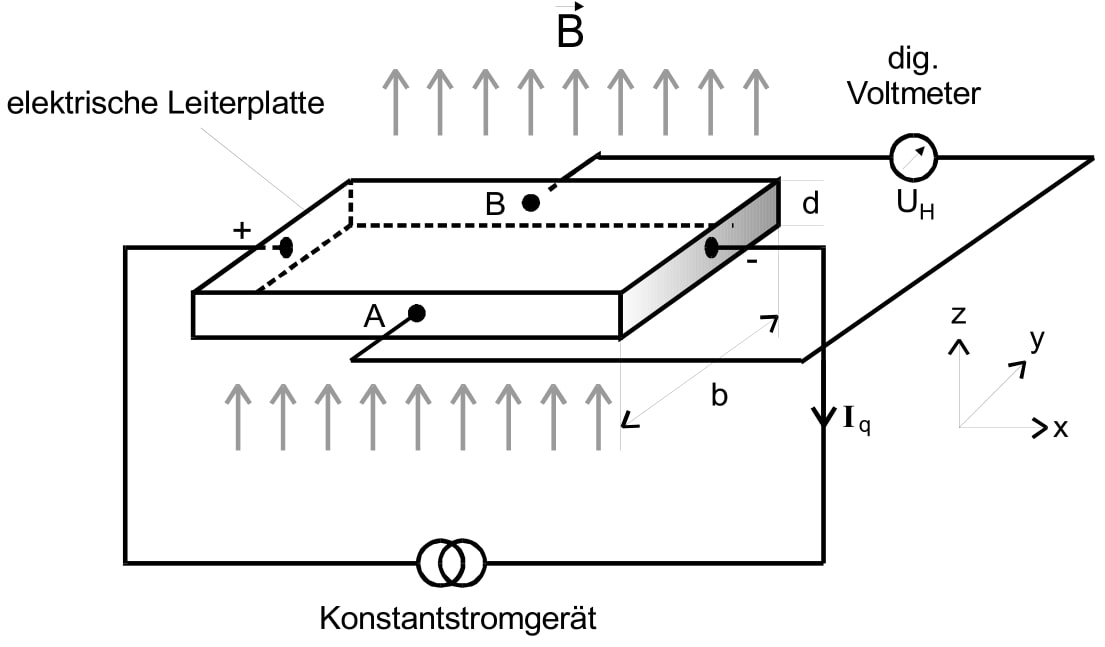
\includegraphics[width=\linewidth]{./images/leiterplatte.jpg}
    \caption{Aufbau der Leiterplatte \cite{V311}}
    \label{fig:1}
\end{figure}



% Auswertung %%%%%%%%%%%%%%%%%%%%%%%%%%%%%%%%%%%%%%%%%%%%%%%%%%%%%%%%%%%%%%%%%%%%%%%%%%%%%%%%%%%%%%%%%%%%%%%%%%%%%%%%%%%%%%%%%%%%%%%%%%%%%%%%%%%%%%%%%%%%%%%%%%%%%%%%%%%%%%%%%%%%%%%%%%%%%%%%%%%%%%%%%%%%%%%%%%

\section{Auswertung}
% Hysterese ===============================================================================================================================================================================================================

\begin{table}
    \centering
    \input{Hysterese_table.tex}
    \caption{Hysterese des Magnetfelds}
    \label{tab:1}
\end{table}

\begin{figure}[H]
\centering
\includegraphics[width=0.75\linewidth]{./build/plothy.pdf}
\caption{Hysteresekurve}
\end{figure}

% Kupfer ===============================================================================================================================================================================================================

\begin{table}[H]
    \centering
    \input{Cu_table.tex}
    \caption{Hallspannung $U_H$ von Kupfer}
    \label{tab:2}
\end{table}

\begin{figure}[H]
\begin{subfigure}{0.495\linewidth}
\centering
\includegraphics[width=0.75\linewidth]{./build/plotCu_IB.pdf}
\caption{Hallspannung bei konstantem Querstrom}
\end{subfigure}
\begin{subfigure}{0.495\linewidth}
\centering
\includegraphics[width=0.75\linewidth]{./build/plotCu_IQ.pdf}
\caption{Hallspannung bei konstantem B-Feld}
\end{subfigure}
\caption{Hallspannungen für Kupfer}
\end{figure}

% Zink ===============================================================================================================================================================================================================

\begin{table}[H]
    \centering
    \input{Zn_table.tex}
    \caption{Hallspannung $U_H$ von Zink}
    \label{tab:3}
\end{table}

\begin{figure}[H]
\begin{subfigure}{0.495\linewidth}
\centering
\includegraphics[width=0.75\linewidth]{./build/plotZn_IB.pdf}
\caption{Hallspannung bei konstantem Querstrom}
\end{subfigure}
\begin{subfigure}{0.495\linewidth}
\centering
\includegraphics[width=0.75\linewidth]{./build/plotZn_IQ.pdf}
\caption{Hallspannung bei konstantem B-Feld}
\end{subfigure}
\caption{Hallspannungen für Zink}
\end{figure}


% Silber ===============================================================================================================================================================================================================

\begin{table}[H]
    \centering
    \input{Ag_table.tex}
    \caption{Hallspannung $U_H$ von Silber}
    \label{tab:4}
\end{table}

\begin{figure}[H]
\begin{subfigure}{0.495\linewidth}
\centering
\includegraphics[width=0.75\linewidth]{./build/plotAg_IB.pdf}
\caption{Hallspannung bei konstantem Querstrom}
\end{subfigure}
\begin{subfigure}{0.495\linewidth}
\centering
\includegraphics[width=0.75\linewidth]{./build/plotAg_IQ.pdf}
\caption{Hallspannung bei konstantem B-Feld}
\end{subfigure}
\caption{Hallspannungen für Silber}
\end{figure}


% Diskussion %%%%%%%%%%%%%%%%%%%%%%%%%%%%%%%%%%%%%%%%%%%%%%%%%%%%%%%%%%%%%%%%%%%%%%%%%%%%%%%%%%%%%%%%%%%%%%%%%%%%%%%%%%%%%%%%%%%%%%%%%%%%%%%%%%%%%%%%%%%%%%%%%%%%%%%%%%%%%%%%%%%%%%%%%%%%%%%%%%%%%%%%%%%%%%%%%%

\section{Diskussion}


% Literatur %%%%%%%%%%%%%%%%%%%%%%%%%%%%%%%%%%%%%%%%%%%%%%%%%%%%%%%%%%%%%%%%%%%%%%%%%%%%%%%%%%%%%%%%%%%%%%%%%%%%%%%%%%%%%%%%%%%%%%%%%%%%%%%%%%%%%%%%%%%%%%%%%%%%%%%%%%%%%%%%%%%%%%%%%%%%%%%%%%%%%%%%%%%%%%%%%%

\newpage
\printbibliography

\end{document}